\documentclass[compress, blue]{beamer}
%http://www.math.utah.edu/~smith/AmberSmith_GSAC_Beamer.pdf
\usepackage{beamerthemeshadow}
\usepackage{multimedia}
\usetheme{Warsaw} % Beamer Theme
\usepackage{hyperref}
\usepackage{animate}

\useoutertheme[subsection=false]{smoothbars} % Beamer Outer Theme
\useinnertheme{rectangles} % Beamer Inner Them
\usepackage{graphicx}
\setbeamercovered{transparent}
\mode<presentation>

\begin{document}

\title{Go Fish}   
\subtitle{A CS205 Software Engineering Project for Dr. Jason Hibbeler}
\author[Phelan,Josh,Ethan,Scott,Danielle]{Phelan Vanderville \and Joshua Dickerson \and Ethan Eldridge \and Scott MacEwan\and  Danielle Steimke} 
\date{\today} 



\begin{frame}
\maketitle
\end{frame}

\section{Overview}

\begin{frame}{Overview}

\begin{itemize}
\item<1>Credits
\item<2>High Level Game Design
\item<3>Development Process
\item<4>Statistics
\item<5>Game Demonstration
\item<6>Conclusions and the Future
\end{itemize}

\end{frame}

\section{Credit}

\begin{frame}{Credit where credit is due}
\begin{itemize}
\item<1>Team Lead: Phelan Vanderville
\item<1>Human Player Logic: Phelan Vanderville
\item<2>AI Design: Josh Dickerson
\item<2>Card,Deck,Hand classes: Josh Dickerson
\item<3>User Interface: Ethan Eldridge
\item<3>Presentation: Ethan Eldridge
\item<4>Game Loop: Danielle Steimke
\item<5>Card,Deck,Hand refactoring: Scott MacEwan
\item<6>Game Design: Phelan,Josh,Ethan,Scott,Danielle
\end{itemize}
\end{frame}

\section{Game Design}

\begin{frame}{Game Overview}
\begin{center}
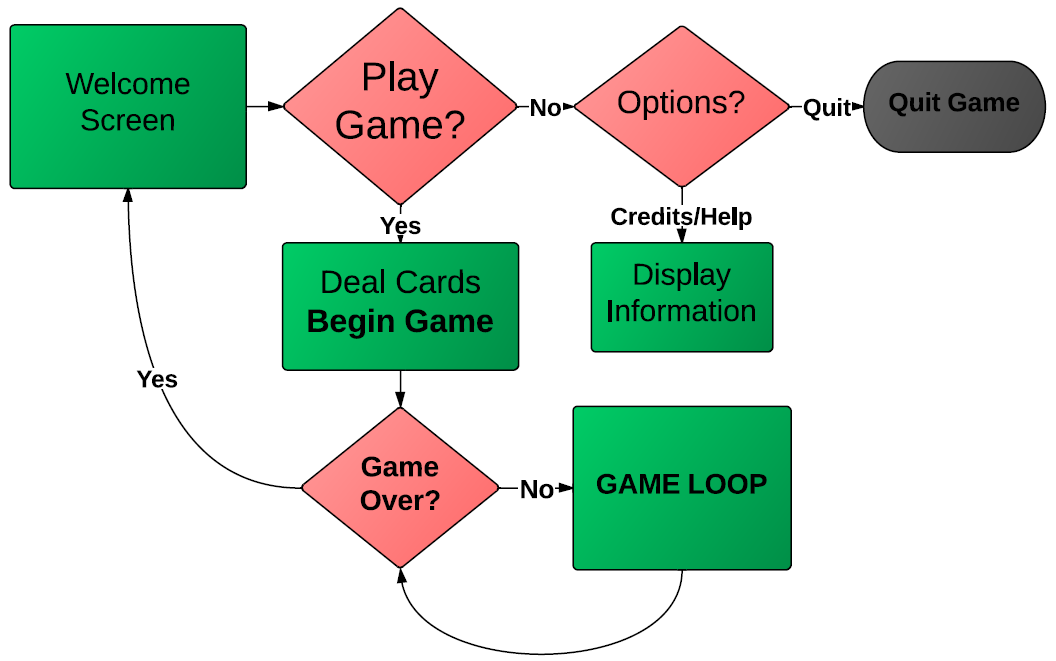
\includegraphics[width=10cm]{Overview.PNG}
\end{center}
\end{frame}

\begin{frame}{Core System Logic}
\begin{center}
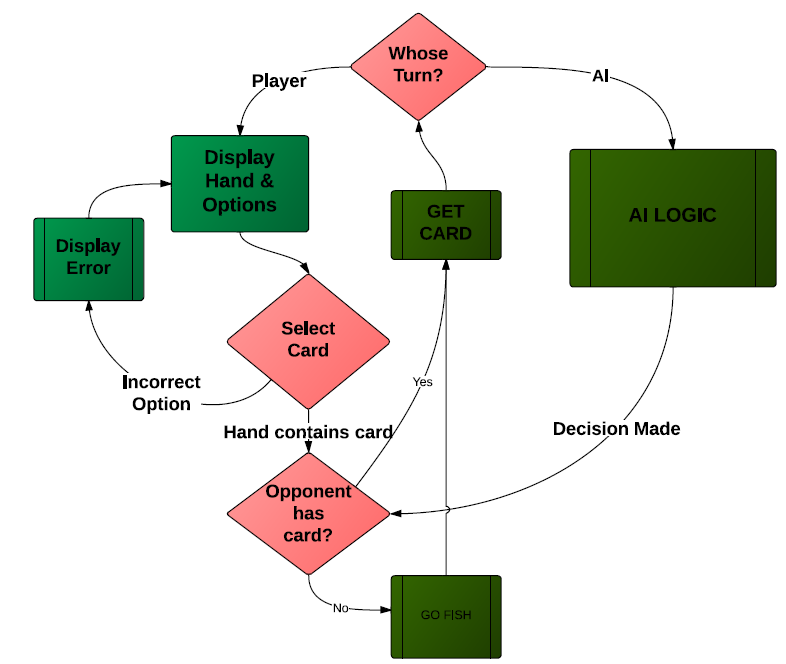
\includegraphics[width=8cm]{CoreLogic.PNG}
\end{center}
\end{frame}



\section{Development Process}

\begin{frame}{Initial Planning}
	\only<1>{
	\begin{itemize}
		\item<1> We all sat down and whiteboarded the overall design
		\item<1> Using Josh's premade classes of Deck,Card, and Hand as a template we planned out interfaces
	 	\item<1> We set up git repositories and remotes to allow for a distributed source
	\end{itemize}
	}

	\only<2>{
	\begin{itemize}
		\item We created a google Drive project specifying
		\begin{itemize}
			\item Contact Information
			\item Areas of Responsibility 
			\item Game Specifications
		\end{itemize}
		\item And set up times to meet and delegation of coding
	\end{itemize}	
	}

	\begin{center}
		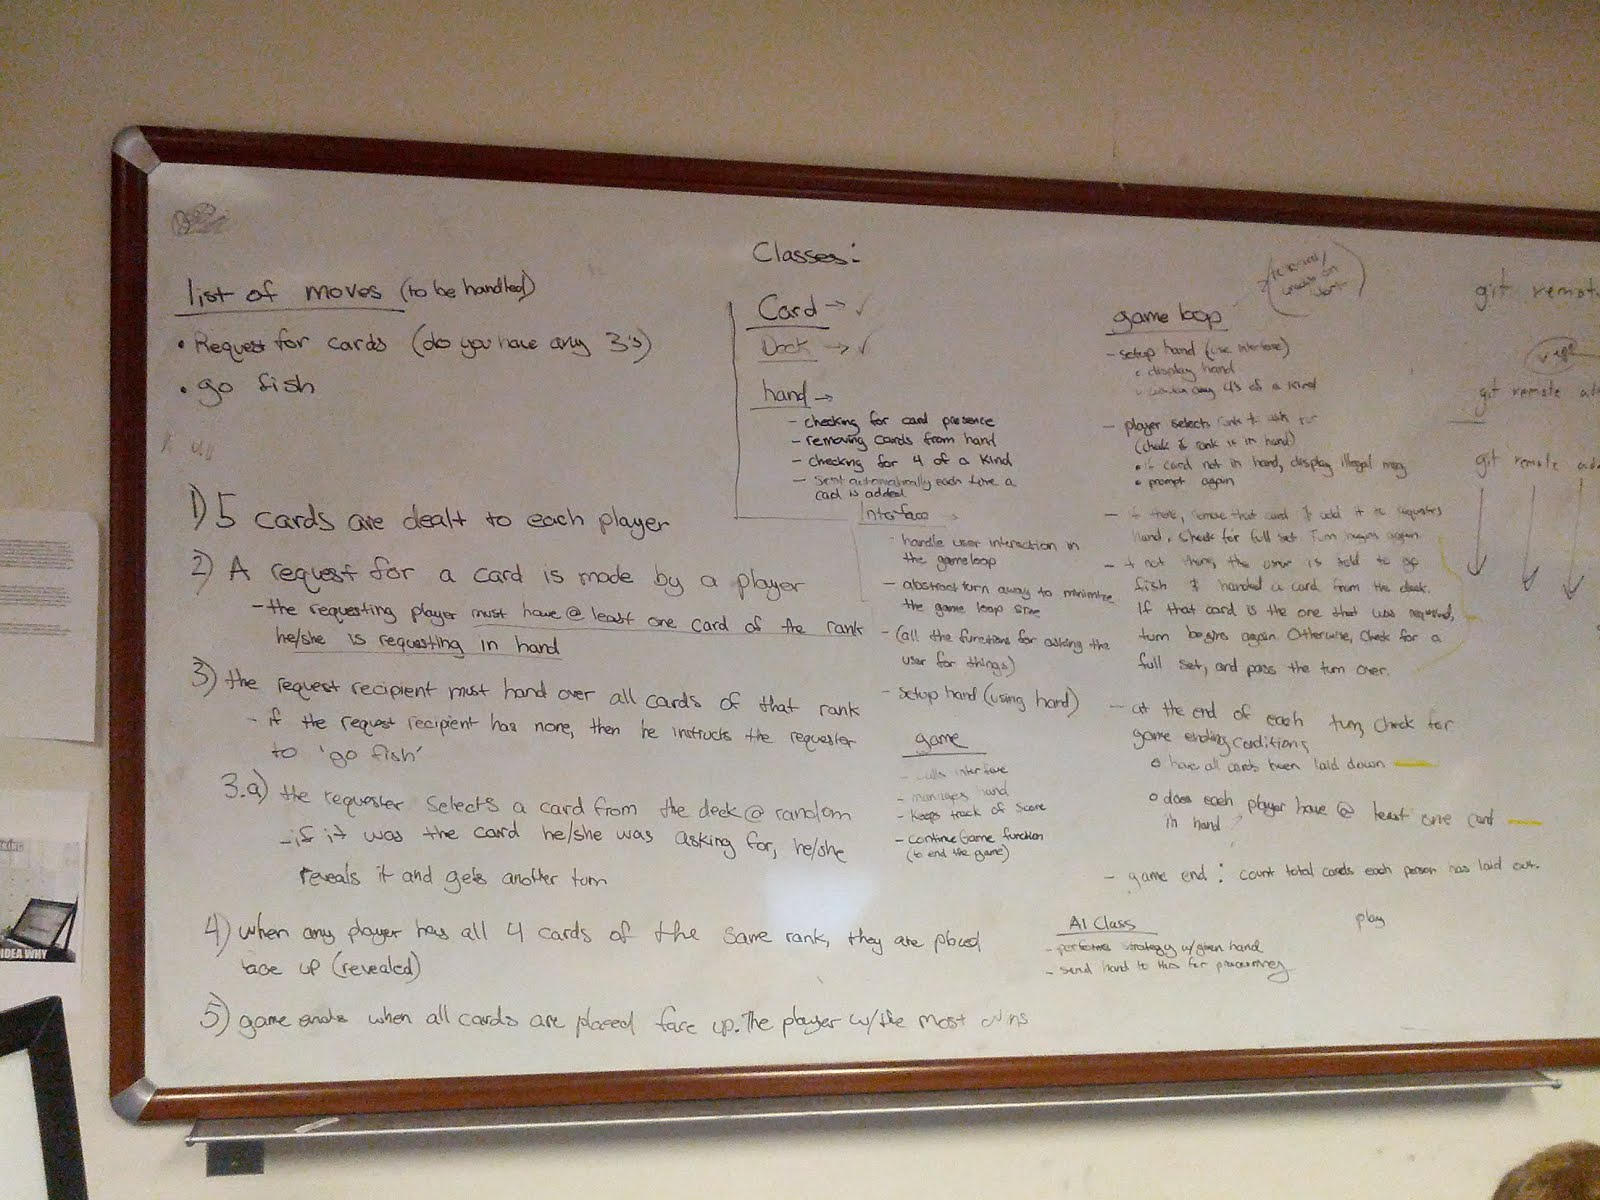
\includegraphics[width=5cm]{whiteboard.jpg}<1-2>
	\end{center}

\end{frame}

\begin{frame}{Developing Code}
	\only<1>{
		\begin{itemize}
			\item We developed our code with a waterfall like specification stage. But an organic iterative implementation loop
			\item A java interface and shell classes guided the flow of the project
			\item At the same time, the code-skeleton allowed enough flexibility to adapt to changing circumstances
		\end{itemize}
	}

	\only<2>{
		\begin{itemize}
			\item Coordination between group members was integral to the process
			\item We used email, chat, github commits and messages, and group coding sessions
			\item Git allowed us to distribute the source and keep up to date iterations amongst the group
		\end{itemize}
	}

	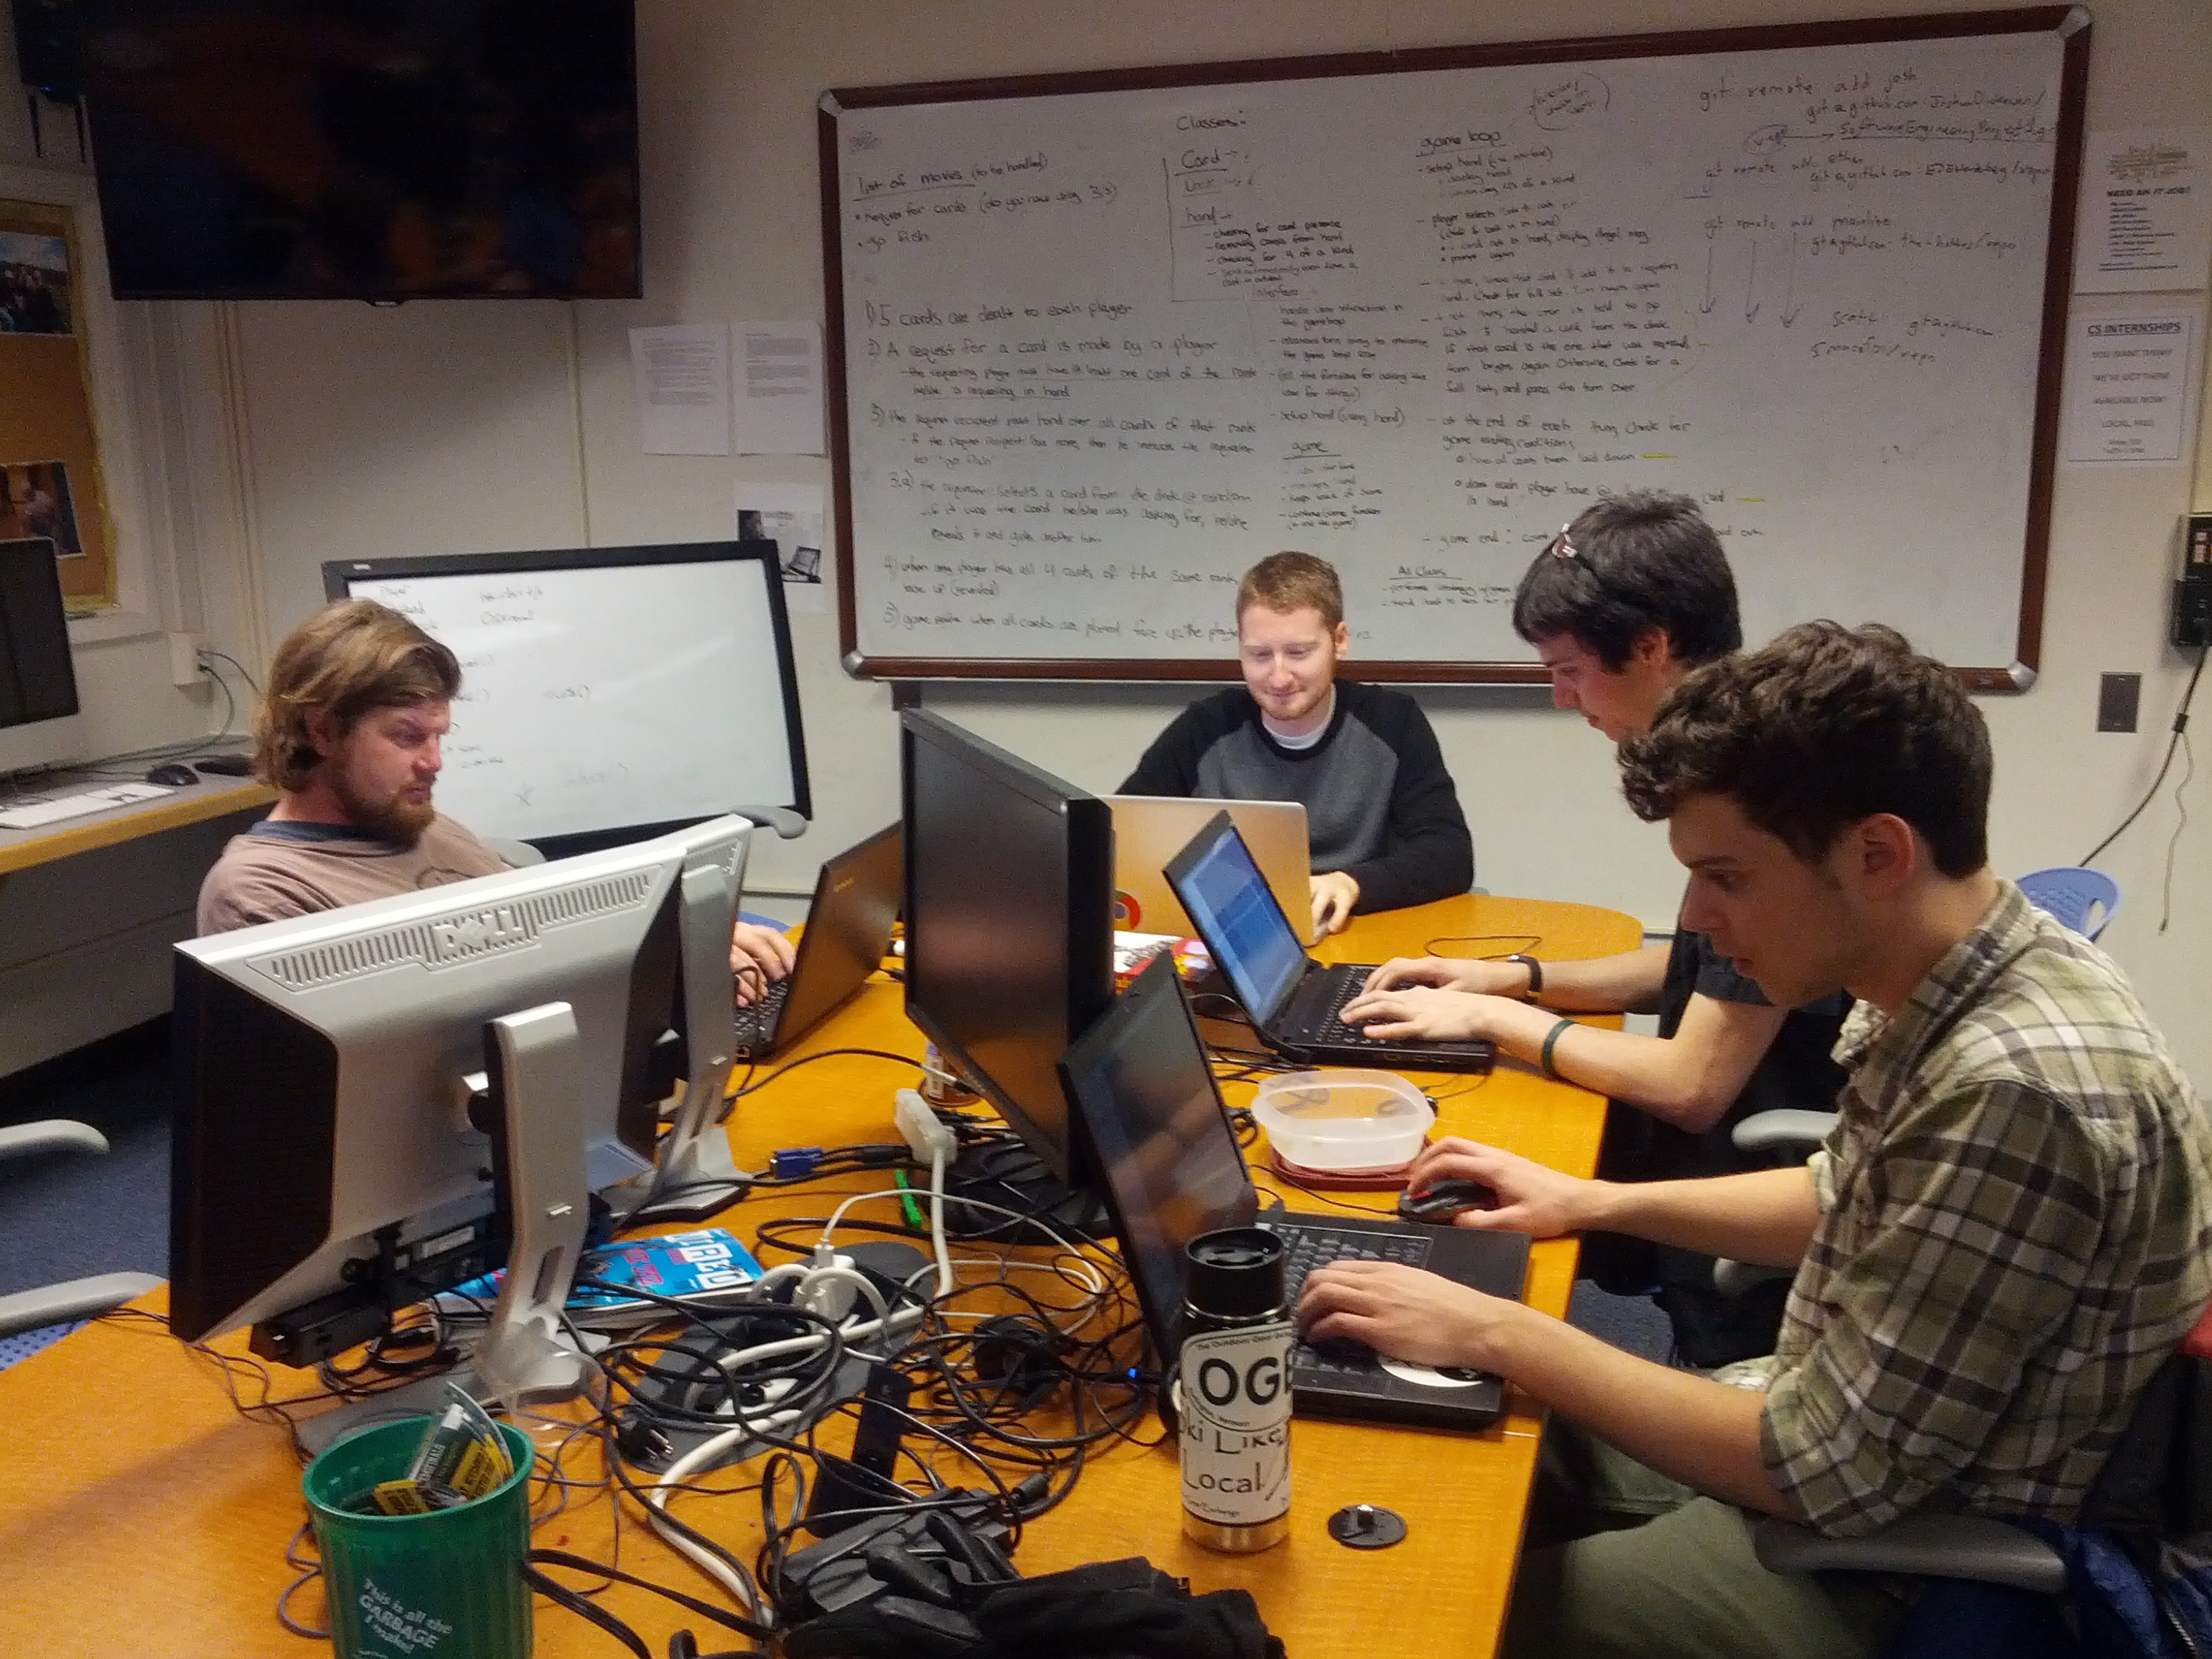
\includegraphics[width=5cm]{coding.jpg}
\end{frame}

\section{Statisics}

\begin{frame}{Statistics}
\begin{itemize}
	\item LAWL WHAT
\end{itemize}
\end{frame}

\section{Demonstration}

\begin{frame}{Demonstration}
Look at our sweet game of go fish!
\end{frame}

\section{Conclusions and the Future}

\begin{frame}{What worked?}

	\begin{itemize}
		\item Planning Ahead
		\item Using Git for code coordination
		\item Group coding sessions
		\item Our Group Dynamic
		\item Agreed on Coding Standards
		\item Code partitioning between members
		\item Communicating with each other
	\end{itemize}

\end{frame}

\begin{frame}{What didn't Work}

	\begin{itemize}
		\item Conflicting Schedules
		\item Learning curve of git for new people for it
		\item Mitigated by having experienced git users in group
		\item Running out of work because of simple game 
	\end{itemize}

\end{frame}
 
\begin{frame}{Things to do next time}

	\begin{itemize}
		\item Work in the same group because this one rocked!
		\item Spend a little more time on planning 
	\end{itemize}

\end{frame}

\end{document}


